La idea trivial de la solución a este ejercicio sería realizar un DFS por cada nodo y para dicho ver al nodo más lejano que puede llegar y este sería el camino maslargo para el nodo por donde se comenzo el DFS. Esta idea el único inconveniente es el alto costo temporal para cuando el árbol tenga gran cantidad de nodos ya que su complejidad temporal esta dada por la expresión O($N(N+E)$) donde $N$ sería la cantidad de nodos del árbol y $E$ las aristas del mismo que por definición de un árbol sería $N-1$ por lo que sustituyen en la expresión inicial nos queda O($2N^2-N$). Pero esta idea del DFS nos va a servir para ver la primera variante de solución.

\subsection{Programación dinámica con DFS}
También en este problema, un buen punto de partida para resolver el problema es rootear el árbol arbitrariamente:
\begin{figure}[h!]
	\centering
	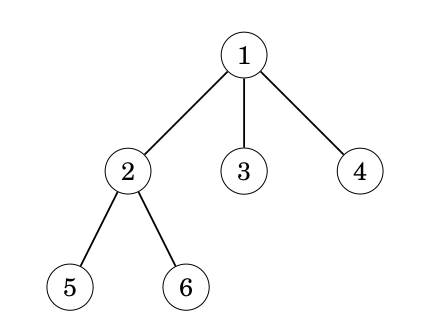
\includegraphics[width=0.4\linewidth]{img/all_longest_paths_2}
	
	\label{fig:alllongestpaths2}
\end{figure}
La primera parte del problema es calcular para cada nodo $x$ la longitud máxima de una ruta que pasa por un hijo de $x$. Por ejemplo, la ruta más larga del nodo $1$ pasa por su hijo $2$:

\begin{figure}[h!]
	\centering
	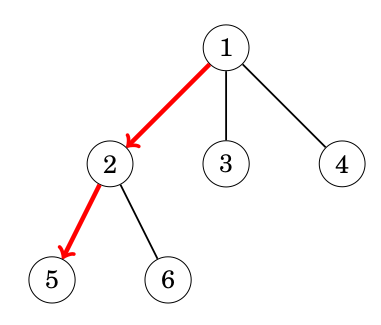
\includegraphics[width=0.4\linewidth]{img/all_longest_paths_3}
	
	\label{fig:alllongestpaths3}
\end{figure}

Esta parte es fácil de resolver en el tiempo O($N$), porque podemos usar la programación dinámica.

Luego, la segunda parte del problema es calcular para cada nodo $x$ la longitud máxima de una ruta a través de su padre $p$. Por ejemplo, la ruta más larga del nodo $3$ pasa por su padre $1$:

\begin{figure}[h!]
	\centering
	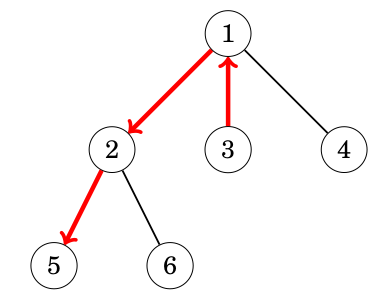
\includegraphics[width=0.4\linewidth]{img/all_longest_paths_4}
	
	\label{fig:alllongestpaths4}
\end{figure}

A primera vista, parece que debemos elegir el camino más largo desde $p$. Sin embargo, esto no siempre funciona, porque el camino más largo de $p$ puede pasar por $x$. Aquí hay un ejemplo de esta situación:

\begin{figure}[h!]
	\centering
	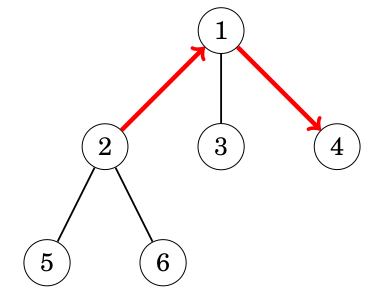
\includegraphics[width=0.4\linewidth]{img/all_longest_paths_5}
	
	\label{fig:alllongestpaths5}
\end{figure}

Aún así, podemos resolver la segunda parte en el tiempo O ($n$) almacenando dos longitudes máximas para cada nodo $x$:

\begin{itemize}
	\item \textbf{$maxLength_1(x)$:} La longitud máxima de una ruta desde $x$
	\item \textbf{$maxLength_2(x)$:} La longitud máxima de una ruta desde $x$ en otra dirección que la primera ruta
\end{itemize}
Por ejemplo, en el anterioranterior, $maxLength_1(1)=2$ usando la ruta $1 \rightarrow 2 \rightarrow 5$, y $maxLength_2(1)=1$ usando la ruta $1 \rightarrow 3$.

Finalmente, si la ruta que corresponde a $maxLength_1(p)$ pasa por $x$, concluimos que la longitud máxima es $maxlength_2(p)+1$, y de lo contrario la longitud máxima es la $maxLength_1(p)+1$.

\subsection{Usando BFS}
Otra idea algorítmica para resolver este problema se basa en la utilización del algoritmo \emph{BFS} con ciertas modificaciones y una estructura como vector o arreglo para almacenar para cada nodo el máximo camino donde él es uno de los extremos.

La idea algorítmica parte del díametro del árbol donde un árbol puede tener uno o varios díametros representados por todos aquellos caminos cuya longitud es máxima en todo el árbol y que comienza en un nodo $u$ y terminan en un nodo $v$. 

Para cualquier nodo $z$ el máximo camino que lo comprende y comienza en él va terminar siempre en un nodo de tipo $u$ o $v$. Por tanto basta con seleccionar un par $(u,v)$ en el árbol y realizar un bfs partiendo sobre cada uno de ellos y ver para cada nodo del árbol de cual de estos dos nodos esta más lejos y ese será el máximo camino para el nodo. Para llevar esta idea vamos a tener dos elementos importantes:

\begin{enumerate}
	\item Un vector o arreglo $path$ con la capacidad igual a la cantidad de nodos con un valor bien pequeño inicialmente. La idea de este vector o arreglo es que voy almacenar en la posición $path[i]$ la longitud máxima de un camino en el árbol donde uno de los extremos de dicho camino es el nodo $i$.
	\item Implementar un \emph{BFS} que retorne el último nodo visitado y que calcule la distancia desde el nodo que se comenzo el \emph{BFS} hacia cualquier otro nodo $i$ del árbol si dicha distancia es mayor que la que se tiene almacenada en el $path$ para el nodo $i$ actualizar el valor de $path[i]$ con dicho valor.
\end{enumerate}

Una vez visto estos detalles el procedimiento sería bien sencillo:

\begin{enumerate}
\item Realizar el \emph{BFS} modificado desde cualquier nodo del árbol escogido de forma arbitraria este nos va devolver un posible nodo $u$.
\item Realizar el \emph{BFS} modificado desde el nodo $u$ obtenido en el paso anterior. Esta ejecucción del \emph{BFS} nos va devolver un posible nodo $v$ asociado con $u$ cuyo camino entre ellos es un diámetro del árbol.
\item Realizar el \emph{BFS} modificado desde el nodo $v$ obtenido en el paso anterior.
 
\end{enumerate}

Una vez realizados estos tres \emph{BFS} en el vector o arreglo $path$ en la posición $i$ tenemos el valor de la longitud del máximo que comienza o termina en el nodo $i$. 

